\documentclass[12pt,a4paper,titlepage]{article}

\usepackage{preamble}

\title{Problème inverse en ElectroEncéphaloGraphie (EEG)}
\author{Saâd Aziz Alaoui, Yassine Jamoud, Samy Haffoudhi}
\date{\today}

\begin{document}

\maketitle

\section*{Introduction}

% sv pour accélèrer inversion (inverse des élements diagnoaux à la place du calcul entier)
% contrairement aux autres méthodes le filtre de tykinov n'a pas besoin de s

Lors de ce TP, nous allons nous intéresser à un exemple de problème
inverse dans le domaine biomédical : la localisation de sources en EEG.
Nous allons reconstruire l'activité à partir de mesures en surface par
les capteurs EEG.

On adopte la modélisation suivante :

$$ x(t) = G s(t) + n(t) $$

Avec,

\begin{itemize}
    \item{$ G \in \mathbb{R^{N \times D}} $}
    \item{N, le nombre de capteurs}
    \item{D, le nombre de dipôles de l'espace source}
    \item{$ x(t) \in \mathbb{R^N} $, le vecteur de mesures}
    \item{$ s(t) \in \mathbb{R^D} $, le vecteur de signal}
    \item{$ n(t) \in \mathbb{R^N} $, un vecteur de bruit}
\end{itemize}

Nous sommes face à un problème inverse linéaire et sous-déterminé
puisque $N \ll D$. Il convient alors de formuler des hypothèses
supplémentaires sur les sources pour obtenir une solution unique.
On utilisera dans ce TP la régularaisation de Tikhonov.

\section{Génération de données}

On travaille sur les données suivantes :

\begin{itemize}
    \item{$ D = 19626 $}
    \item{$ N = 91 $}
    \item{$ T = 200 $ échantillons}
    \item{Les signaux génèrrés proviennent de deux régions sources décarrelées}
    \item{Le bruit est gaussien}
\end{itemize}

Affichons les signaux EEG pour 32 des 91 électrodes :

\begin{figure}[H]
    \caption{Signaux EEG bruités}
    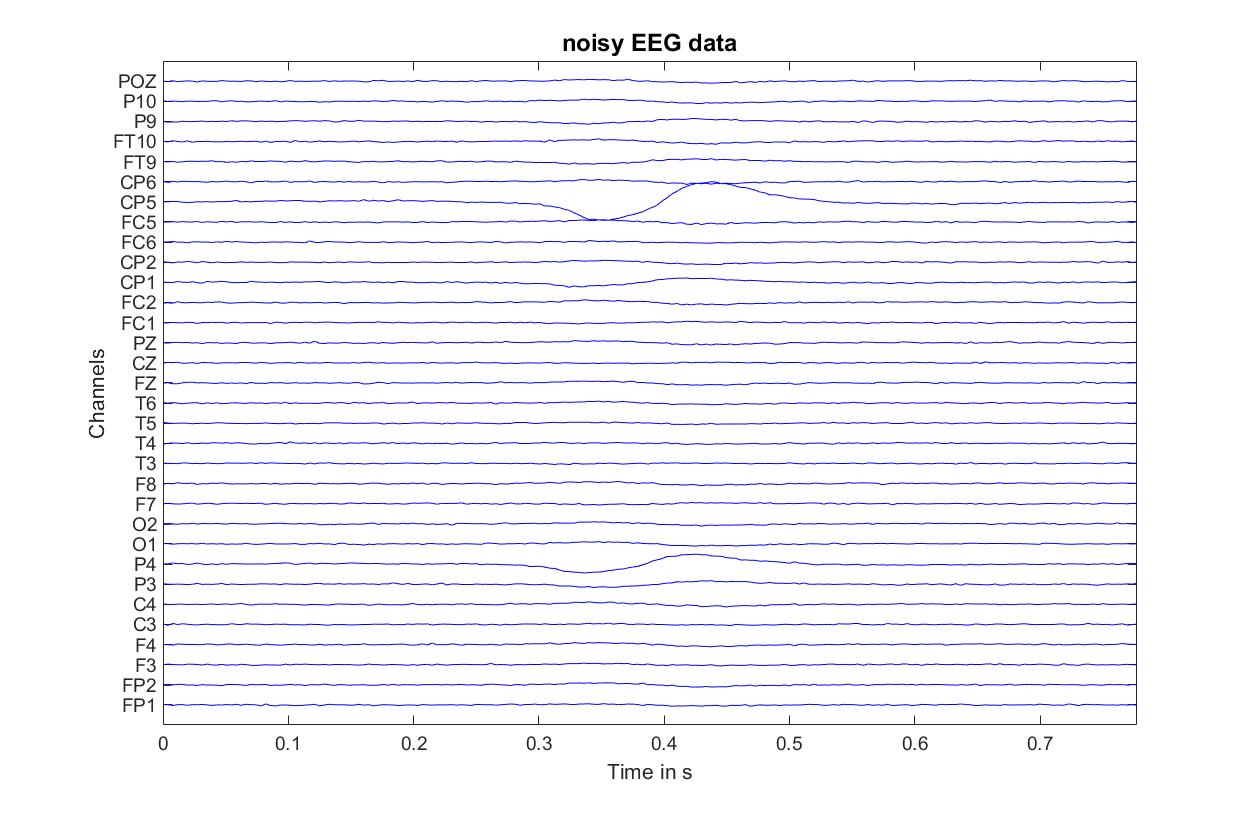
\includegraphics[width=.7\textwidth]{noisyEEG}
    \centering
\end{figure}

Et l'activité des dipoles de l'espace source :

\begin{figure}[H]
    \caption{Activité des dipôles}
    \label{brain}
    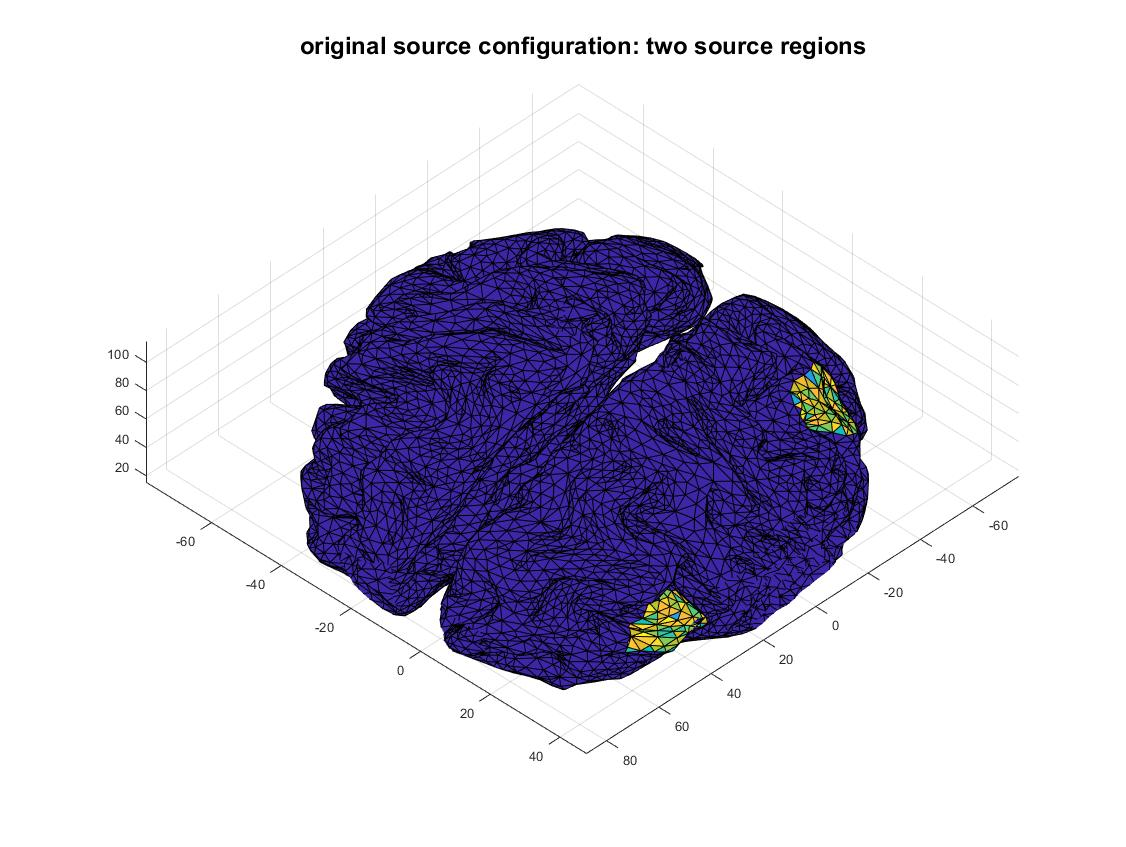
\includegraphics[width=.7\textwidth]{3dbrain}
    \centering
\end{figure}

On observe sur ces données des zones épileptiques quasiment similaires
ainsi qu'une activité de fond gaussienne.

Sur la figure \ref{brain}, on observe bien les deux régions sources
d'où proviennent les signaux générés. Nous allons comparer les résultats
obtenus plus tard à cette vérité terrain.

\section{Régularisation de Tikhonov}

La régularisation de Tikhonov consiste à ajouter un terme de régularisation
en norme 2 pour obtenir le problème d'optimisation suivant :

$$ \min \lVert x - Gs \rVert^2_2 + \lambda \lVert s \rVert^2_2 $$

Avec $\lambda$, un paramètre de régularisation et qui permet d'ajuster
le compromis entre l'adéquation au données et les hypothèses faites sur
la source.

On peut montrer par un calcul du gradient que la solution analytique vaut:

$$ s = G^t(GG^t + \lambda)^{-1}x $$

\textbf{Remarque :} Pour optimiser les calculs on passe par une décomposition en valeurs singulières,
ce qui nous permet d'optimiser l'inversion puisqu'elle revient alors simplement
à inverser les coefficients diagonaux.

Par exemple, pour un rapport signal sur bruit égal à 10, affichons la
DLE (Distance Localisation Error)  en fonction de la valeur du
paramètre $\lambda$ :

\begin{figure}[H]
    \caption{RSB = 10}
    \label{lambdas}
    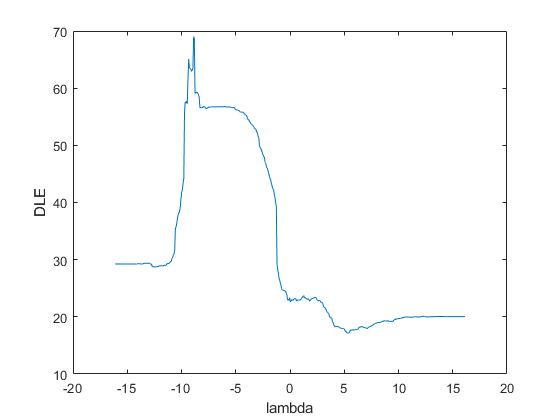
\includegraphics[width=.6\textwidth]{dle_lambda_03}
    \centering
\end{figure}

On balaye une large bande de valeurs du paramètre $\lambda$ et on
sélectionne celle qui permet de minimiser l'erreur DLE. En plus de la large
bande de fréquence il faut également s'assurer d'avoir une période d'échantillonnage
assez faible mais le temps de calcul sera donc plus élevé.

Affichons le résultat obtenu pour la valeur optimale de $\lambda$
pour trois valeurs différentes du RSB sans utiliser de seuil dans un premier
temps :

\begin{figure}[H]
    \caption{RSB = 0.1}
    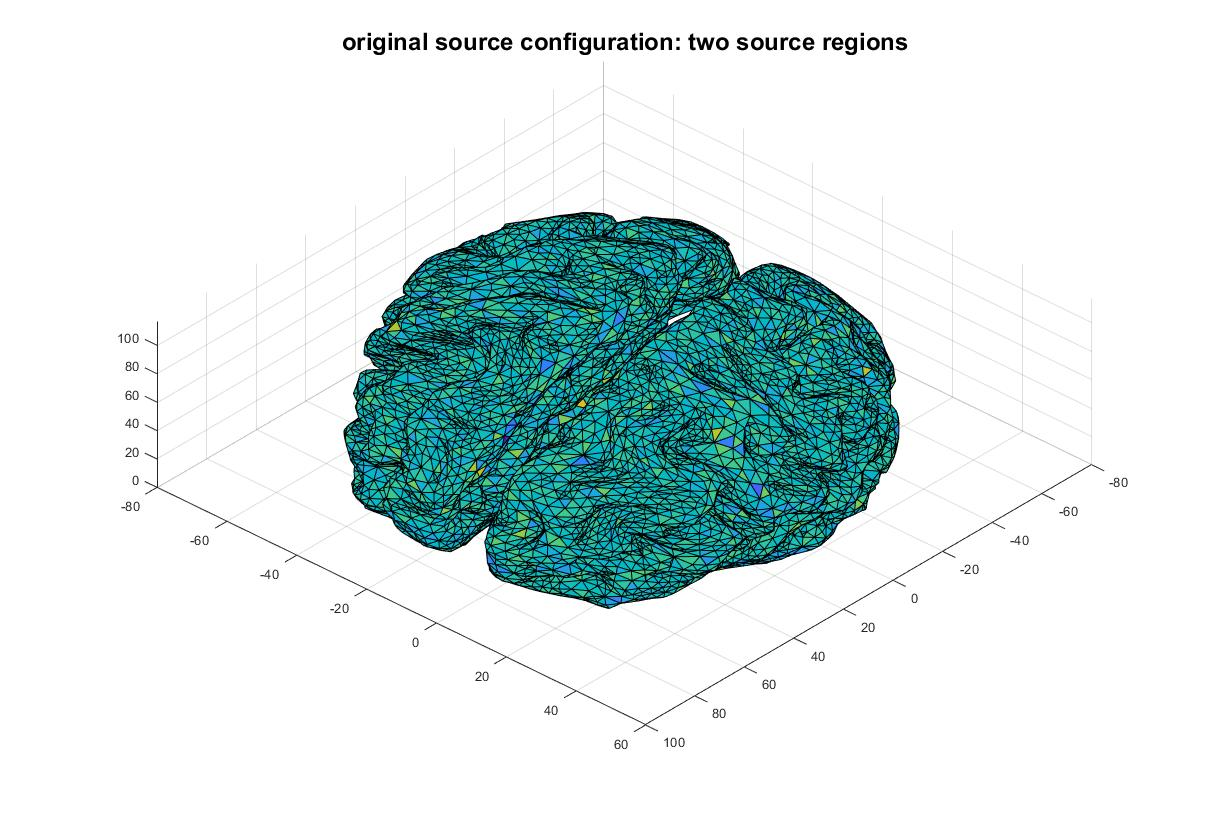
\includegraphics[width=.6\textwidth]{03_01_lambda_opti}
    \centering
\end{figure}

\begin{figure}[H]
    \caption{RSB = 10}
    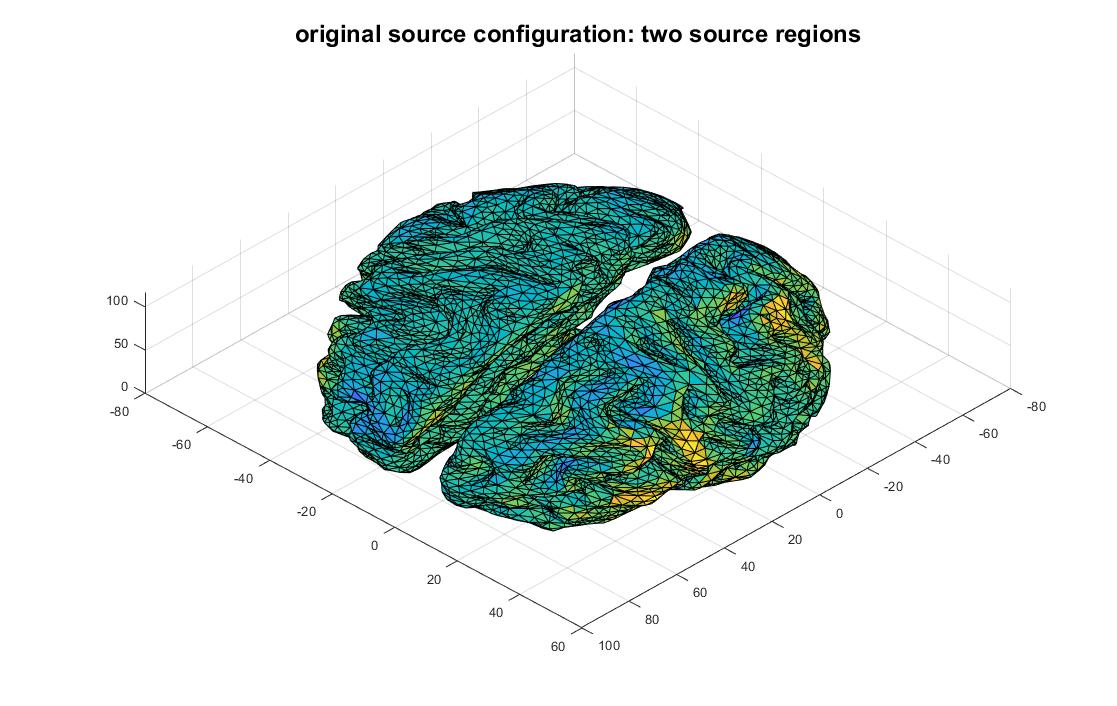
\includegraphics[width=.6\textwidth]{03_10_lambda_opti}
    \centering
\end{figure}

\begin{figure}[H]
    \caption{RSB = 100}
    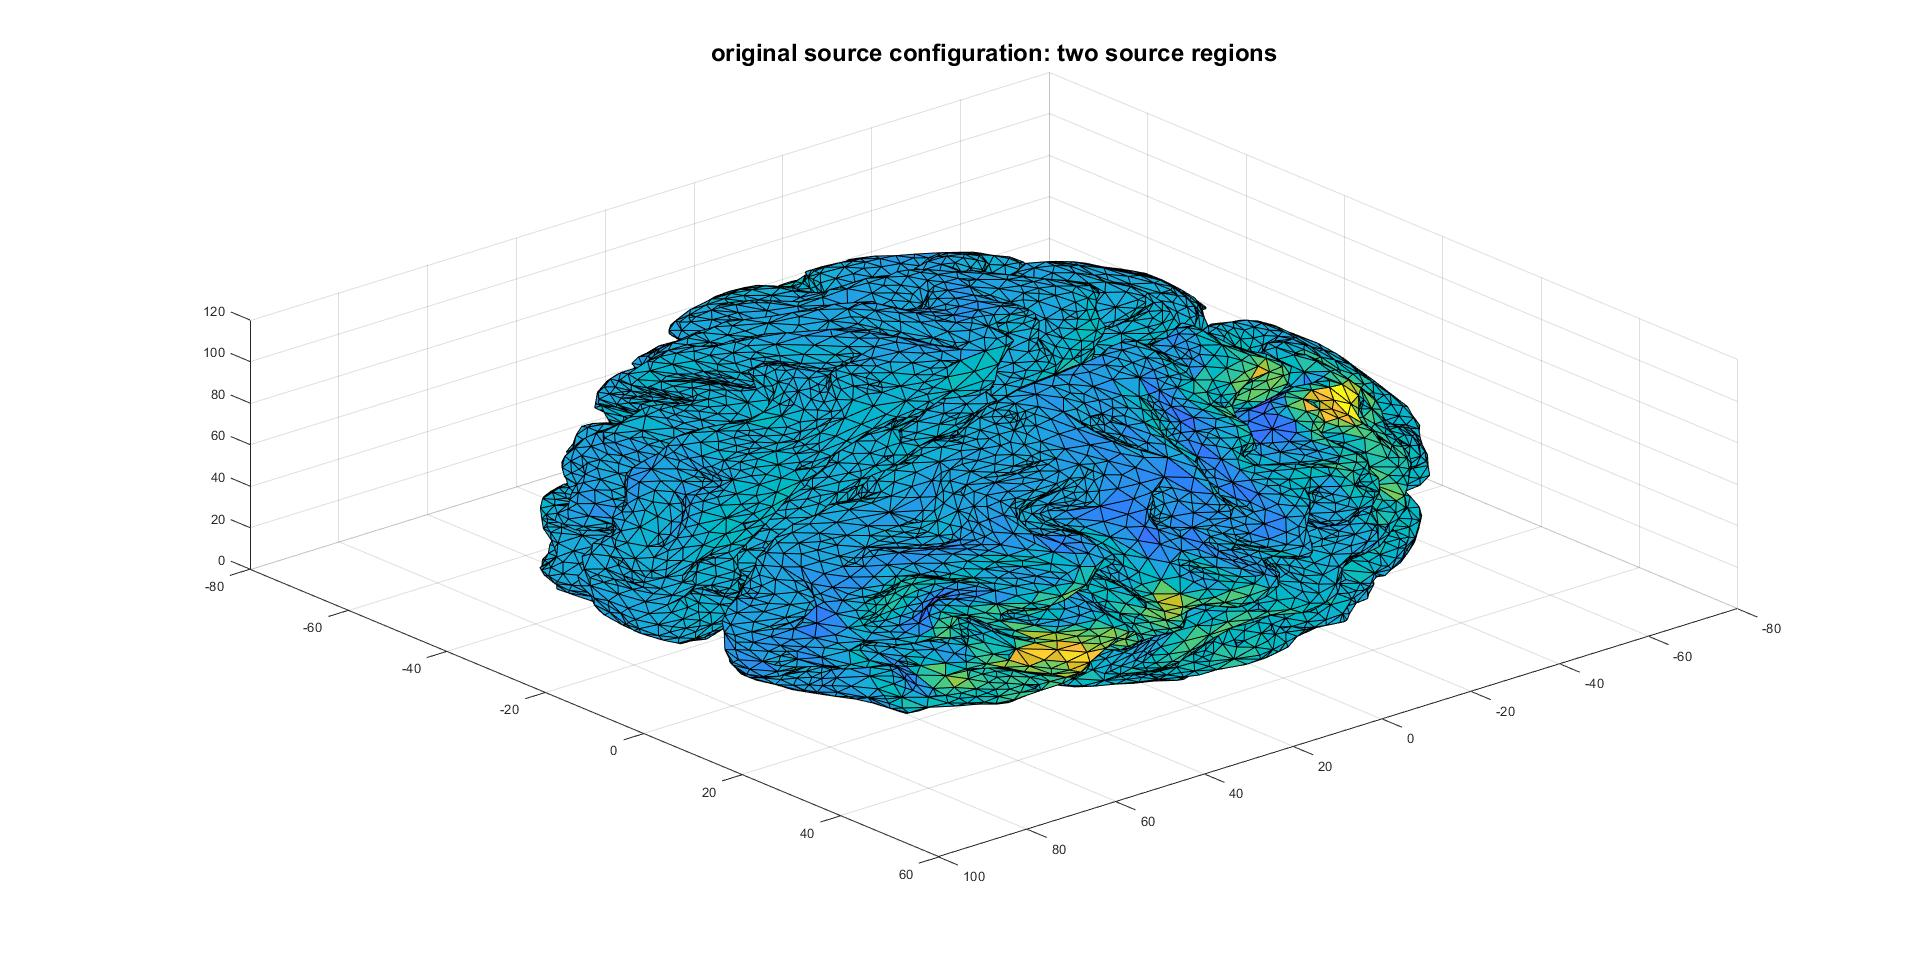
\includegraphics[width=.6\textwidth]{03_100_lambda_opti}
    \centering
\end{figure}

On obtient les valeurs suivantes :

\begin{itemize}
    \item{Pour un $RSB = 0.1$, $ \lambda_{opti} = 3.3 \times 10^{-5} $}
    \item{Pour un $RSB = 10$, $ \lambda_{opti} = 4298 $}
    \item{Pour un $RSB = 100$, $ \lambda_{opti} = 801 $}
\end{itemize}

On observe bien que :

\begin{itemize}
    \item{Plus on a de bruit, moins le résultat est proche de la vérité terrain.
        Pour RSB = 0.1, on ne distingue pas les sources, pour RSB = 10, on commence à distiguer
        les sources mais le résultat le plus proche est obtenu pour RSB = 100}
    \item{Les valeurs retournées pour $\lambda_{opti}$ différent entre les trois RSB et de manière non ordonnée,
        on ne peut donc pas exhiber un lien simple entre RSB et valeur de $\lambda_{opti}$.}
    \item{Comme on le voit par exemple sur la figure \ref{lambdas}, le choix de ce paramètre
        influe grandement sur la valeur DLE obtenue. Il faut donc faire attention à choisir une bonne valeur du paramètre
        si on veut obtenir des bons résultats.}
\end{itemize}

On peut par ailleurs noter l'influence du seuil sur le résultat. Les figures obtenues ci-dessus
ont été tracé sans seuillage. Par exemple pour un seuil égal à 0.9 on serait alors sélectif
et on obtient la figure suivante :

\begin{figure}[H]
    \caption{RSB = 10 et seuil de 0.9}
    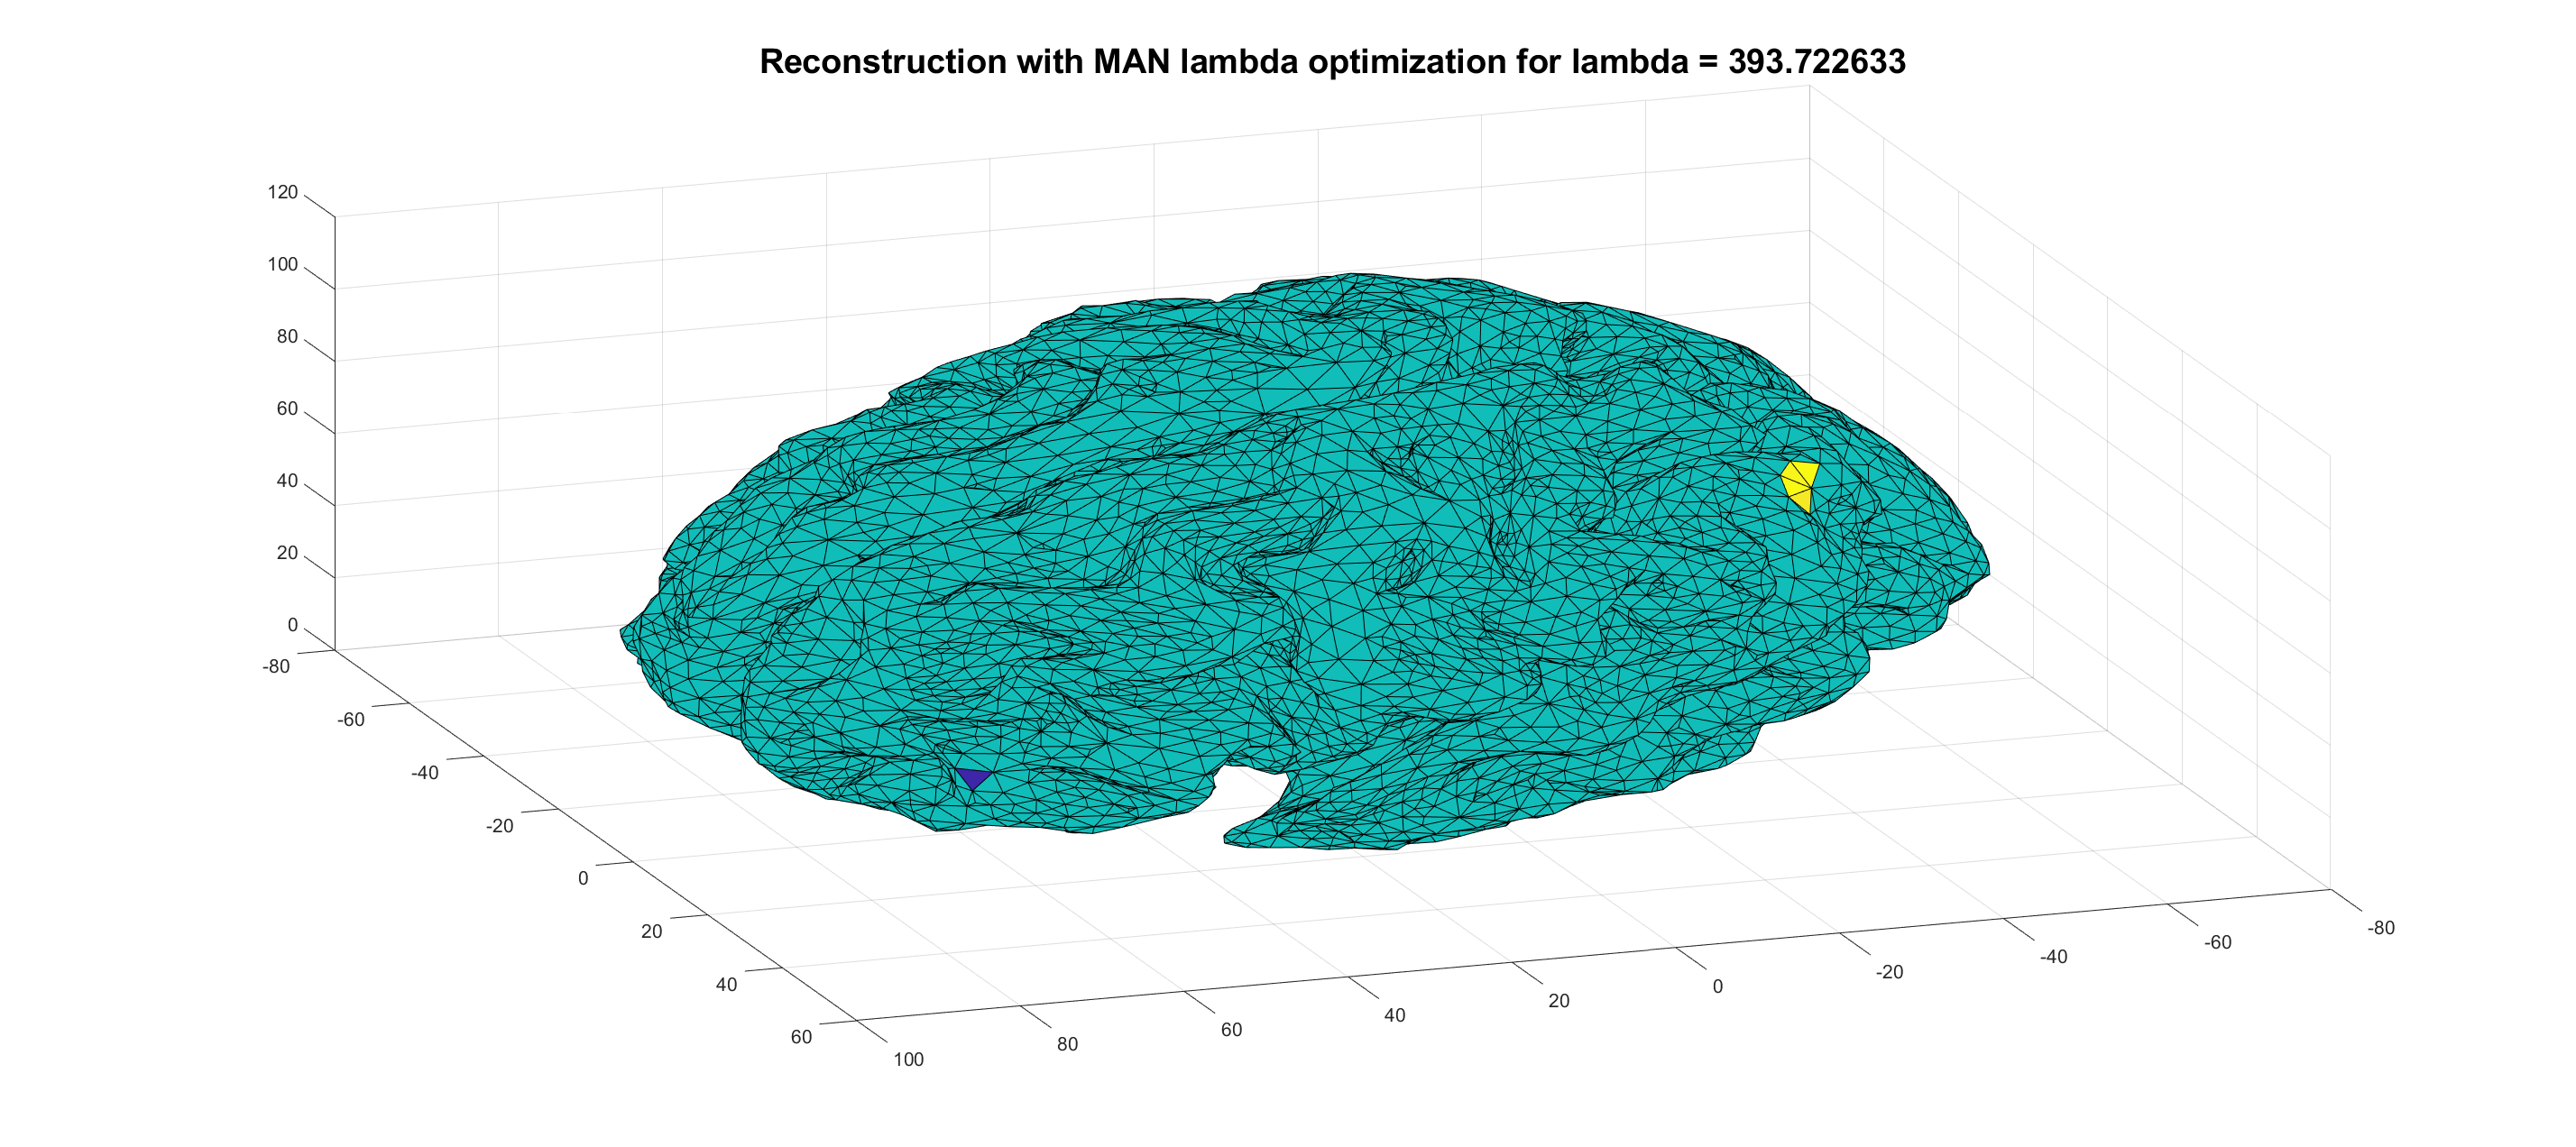
\includegraphics[width=.6\textwidth]{seuil_09}
    \centering
\end{figure}

Le seuil est alors également un paramètre à ajuster.

\section{L-curve}

Pour obtenir la meilleure valeur de $\lambda$,  on exploite alors
la L-Curve. Il s'agit du tracé de la norme de la solution en fonction
de la norme du résidu avec $\lambda$ comme paramètre.

On choisir la valeur de $\lambda$ situé dans le coin de la L-curve afin d'assurer un bon
compromis entre les deux errreurs à minimiser.

Par exemple pour un RSB égal à 1, on obtient la L-curve suivante ainsi que la localisation
de $\lambda_{opti}$ :

\begin{figure}[H]
    \caption{L-curve}
    \label{brain}
    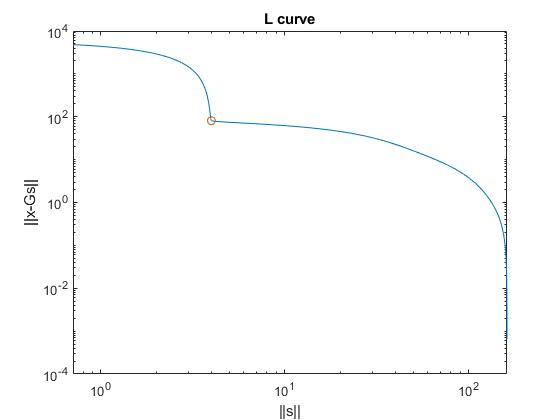
\includegraphics[width=.8\textwidth]{LC}
    \centering
\end{figure}

\section{Comparaison de trois méthodes}

Une autre méthode consiste en l'utilisation du "Discrepacy principle".

Affichons alors les résultats obtenus pour les 3 différentes méthodes pour un RSB égal à 0.1
et pour une même valeur de seuil :

\begin{figure}[H]
    \caption{Méthode manuelle}
    \label{brain}
    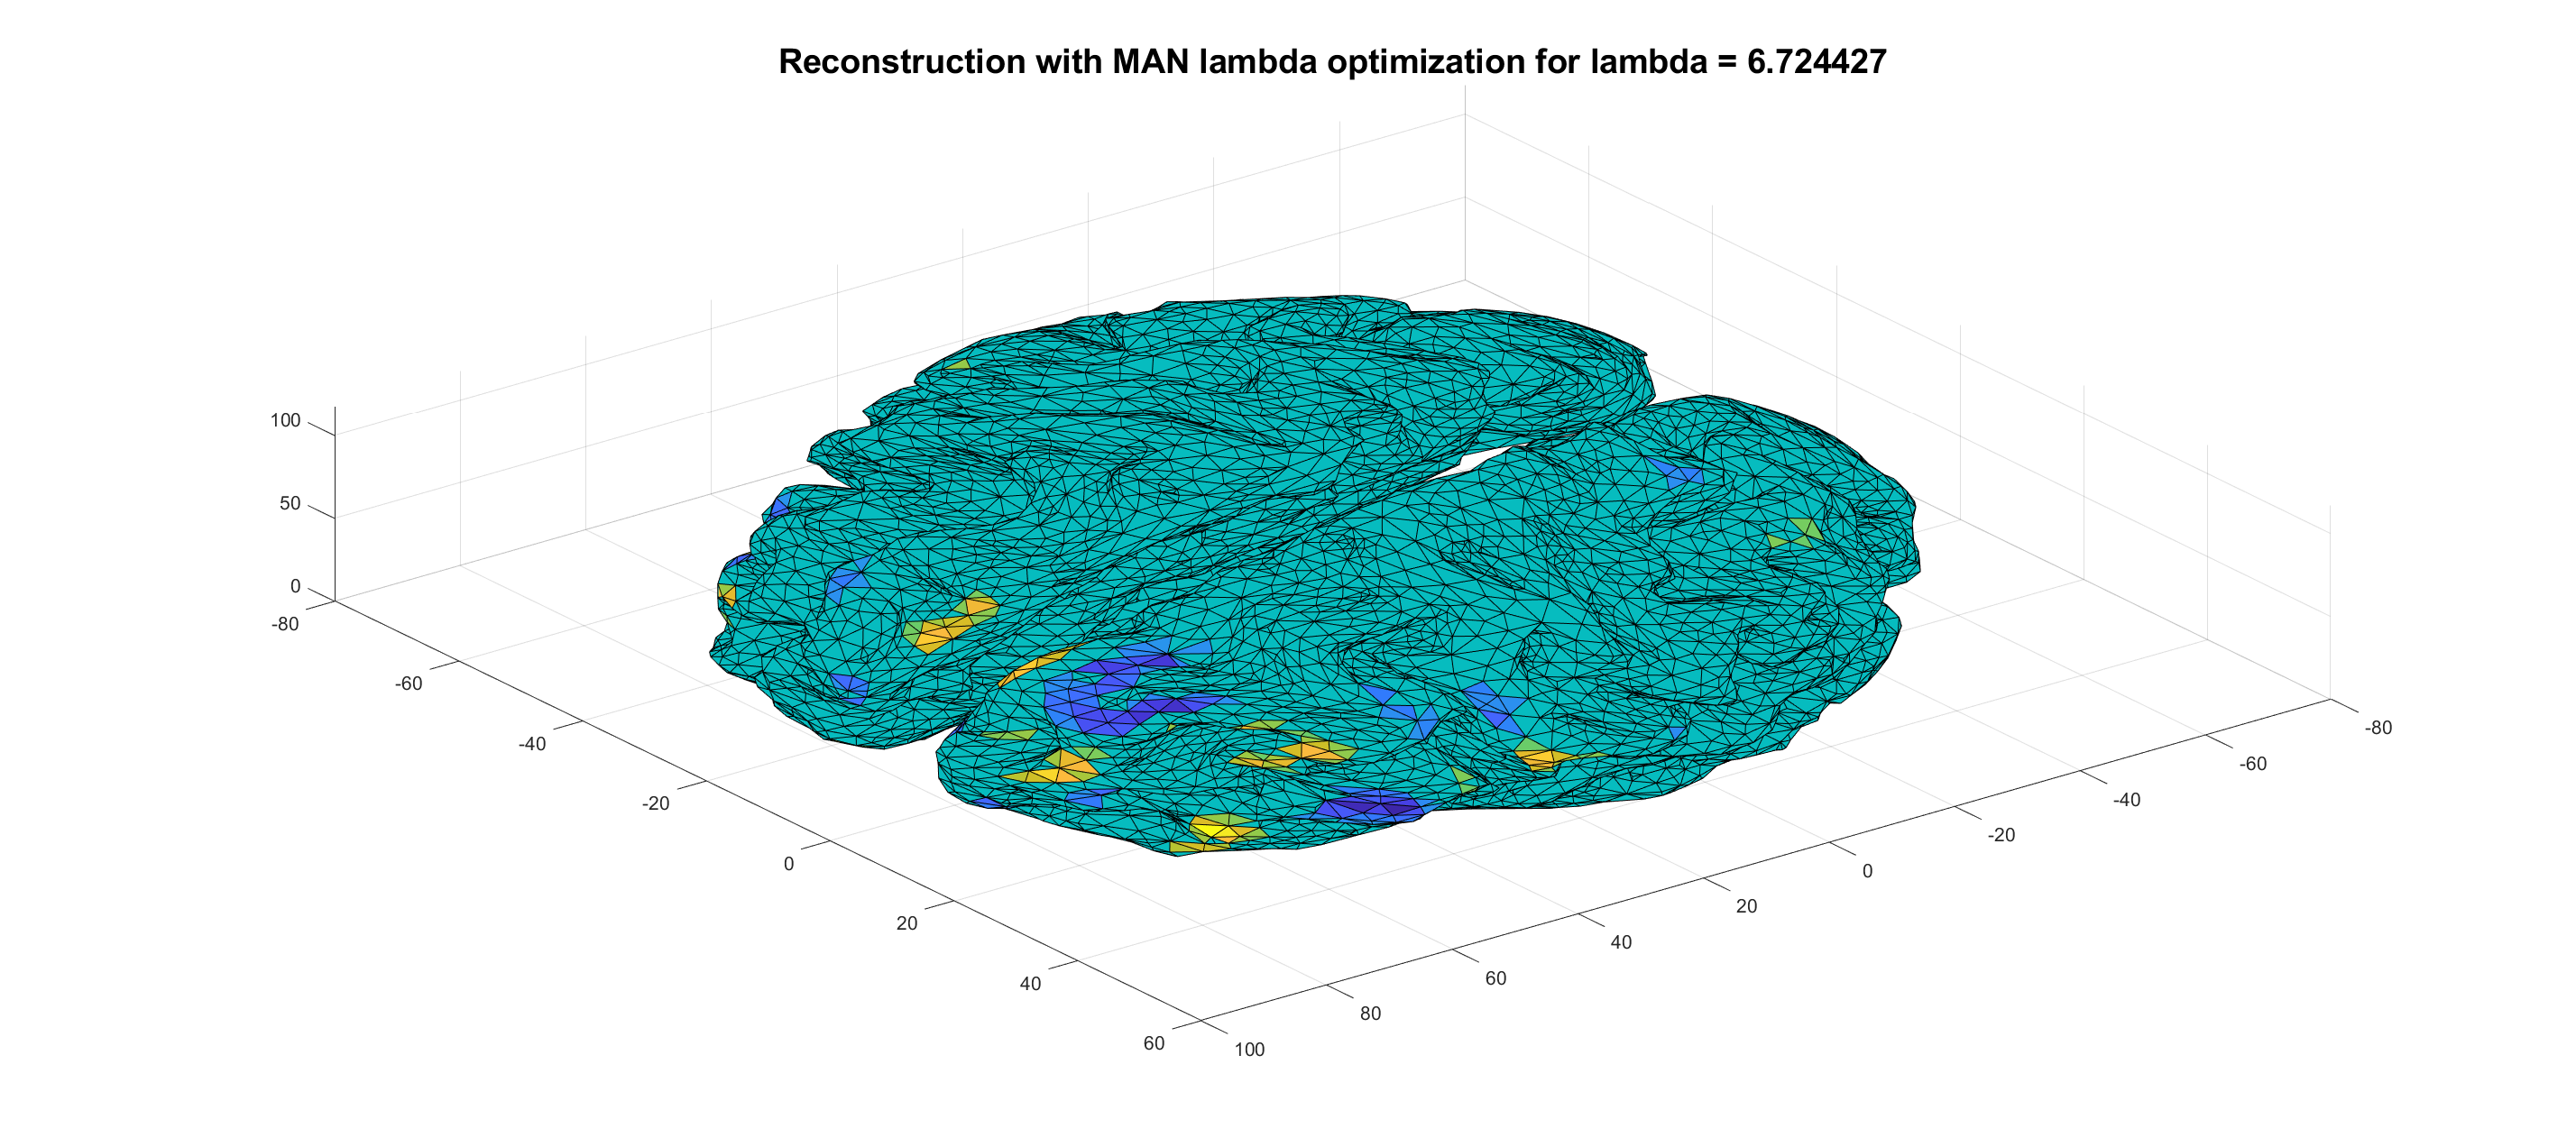
\includegraphics[width=.6\textwidth]{man_01}
    \centering
\end{figure}

\begin{figure}[H]
    \caption{Méthode L-curve}
    \label{brain}
    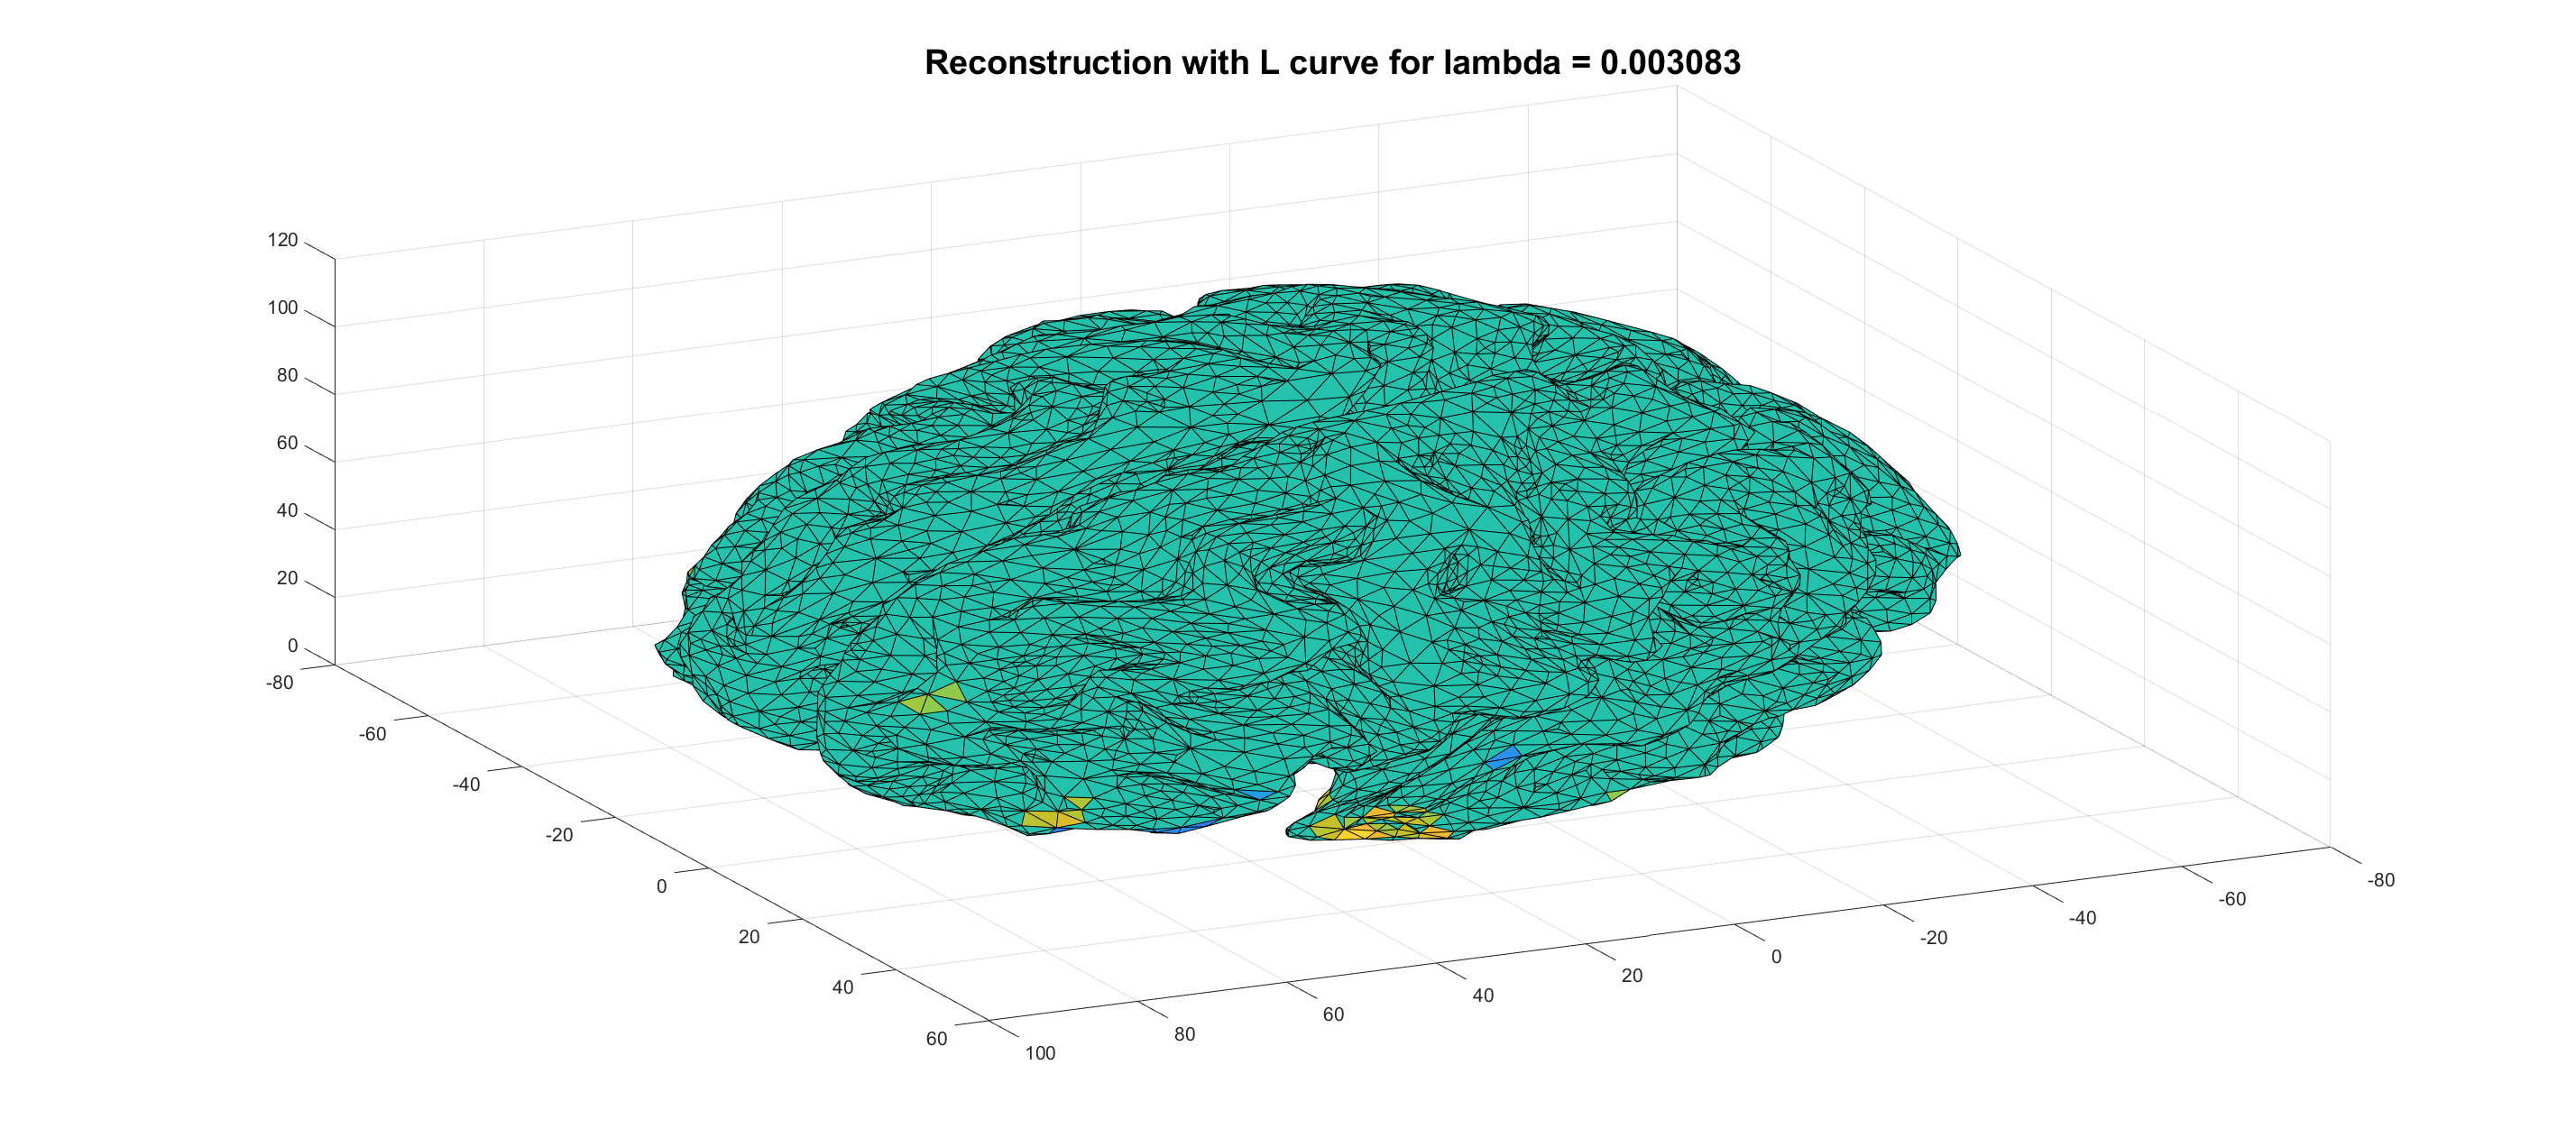
\includegraphics[width=.6\textwidth]{l_01}
    \centering
\end{figure}

\begin{figure}[H]
    \caption{Méthode DISC}
    \label{brain}
    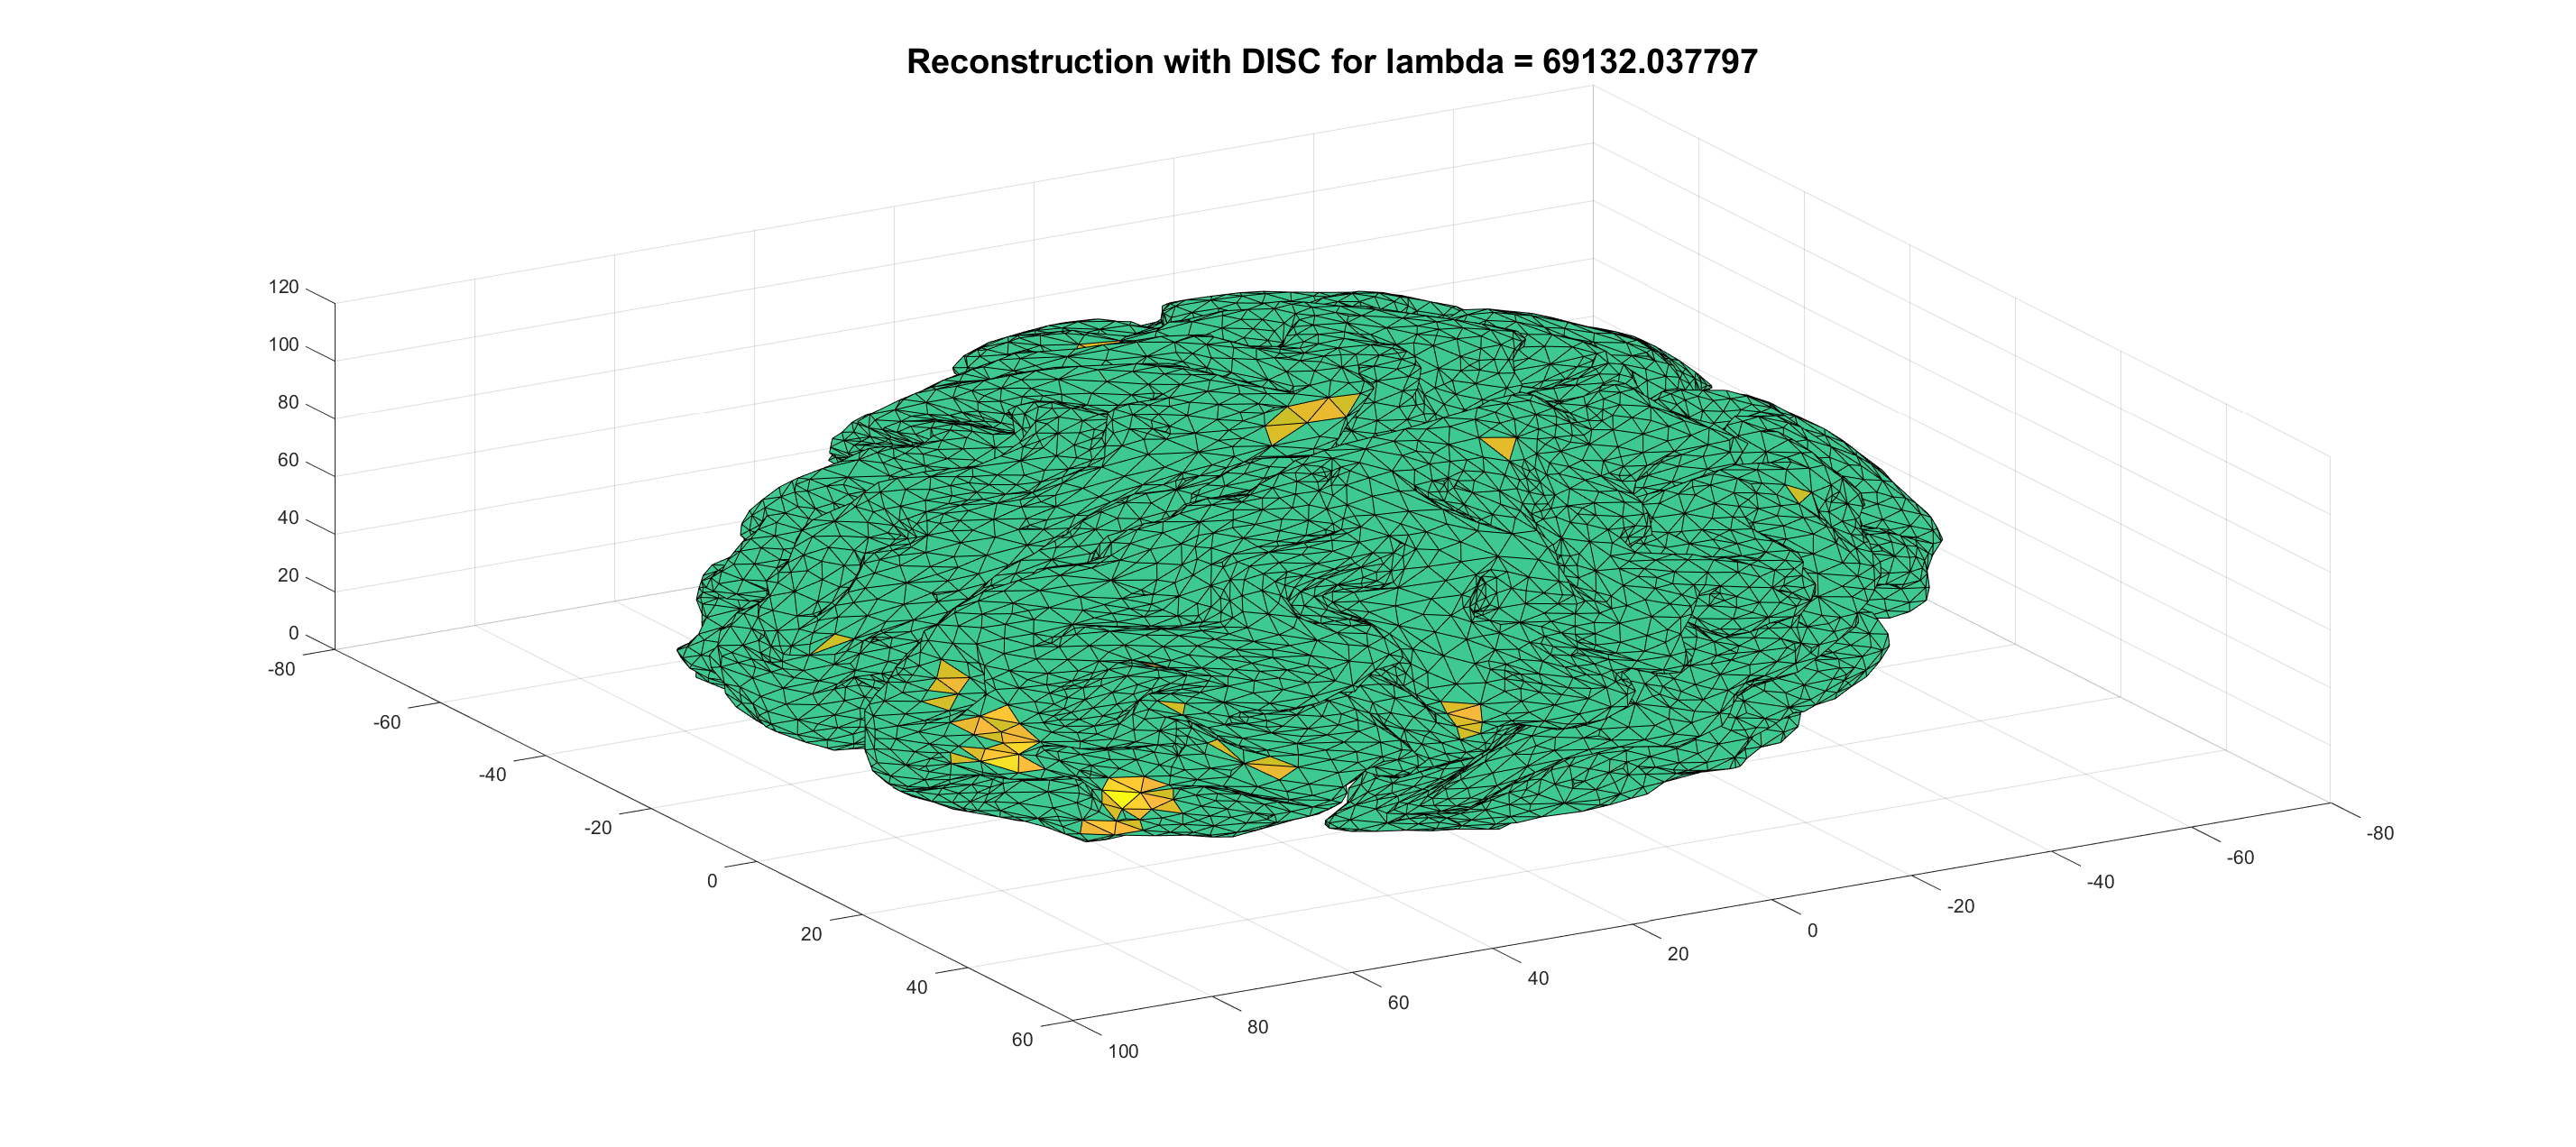
\includegraphics[width=.6\textwidth]{disc_01}
    \centering
\end{figure}

Pour un RSB égal à 10 :

\begin{figure}[H]
    \caption{Méthode manuelle}
    \label{brain}
    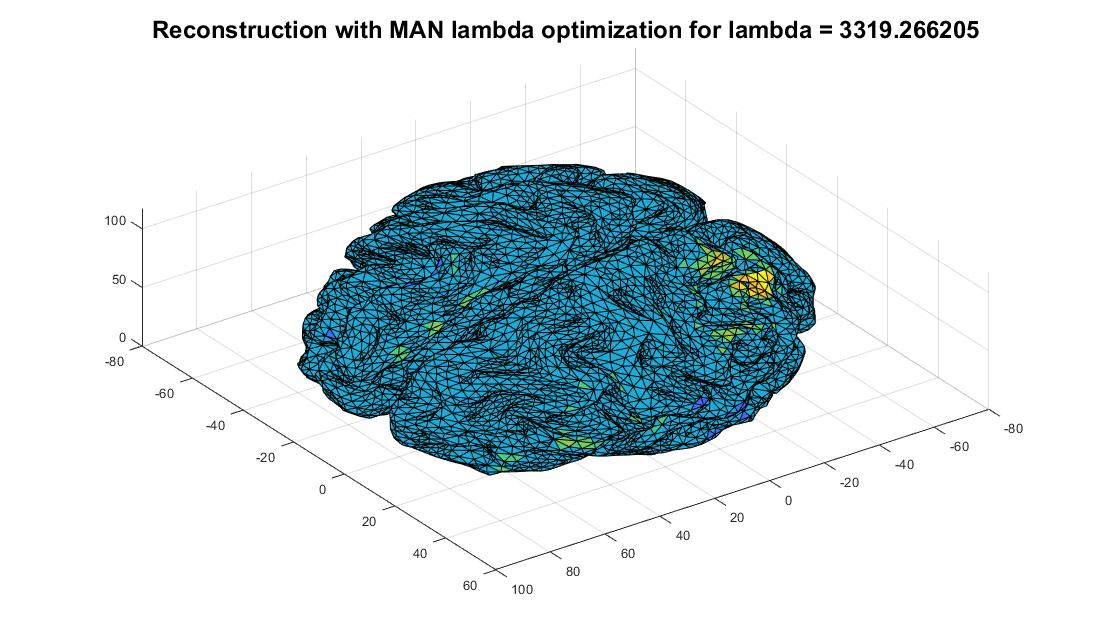
\includegraphics[width=.6\textwidth]{man_seuil}
    \centering
\end{figure}

\begin{figure}[H]
    \caption{Méthode L-curve}
    \label{brain}
    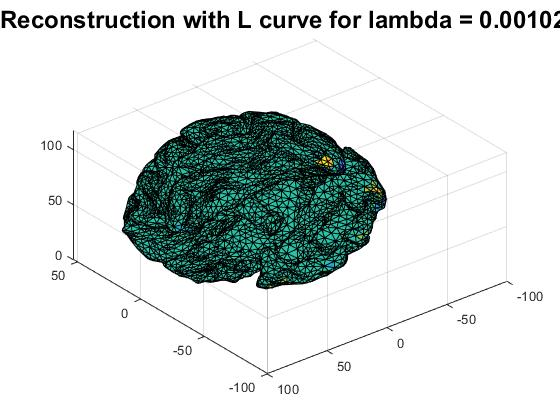
\includegraphics[width=.5\textwidth]{LC_seuil}
    \centering
\end{figure}

\begin{figure}[H]
    \caption{Méthode DISC}
    \label{brain}
    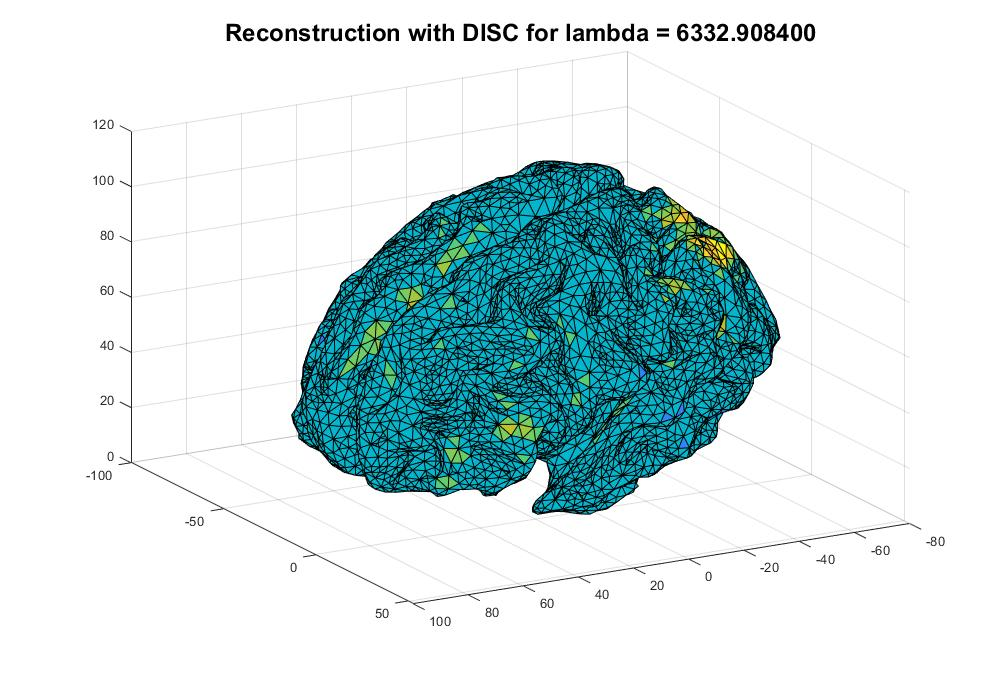
\includegraphics[width=.5\textwidth]{DISC_seuil}
    \centering
\end{figure}

Et enfin, pour un RSB égal à 100 :

\begin{figure}[H]
    \caption{Méthode manuelle}
    \label{brain}
    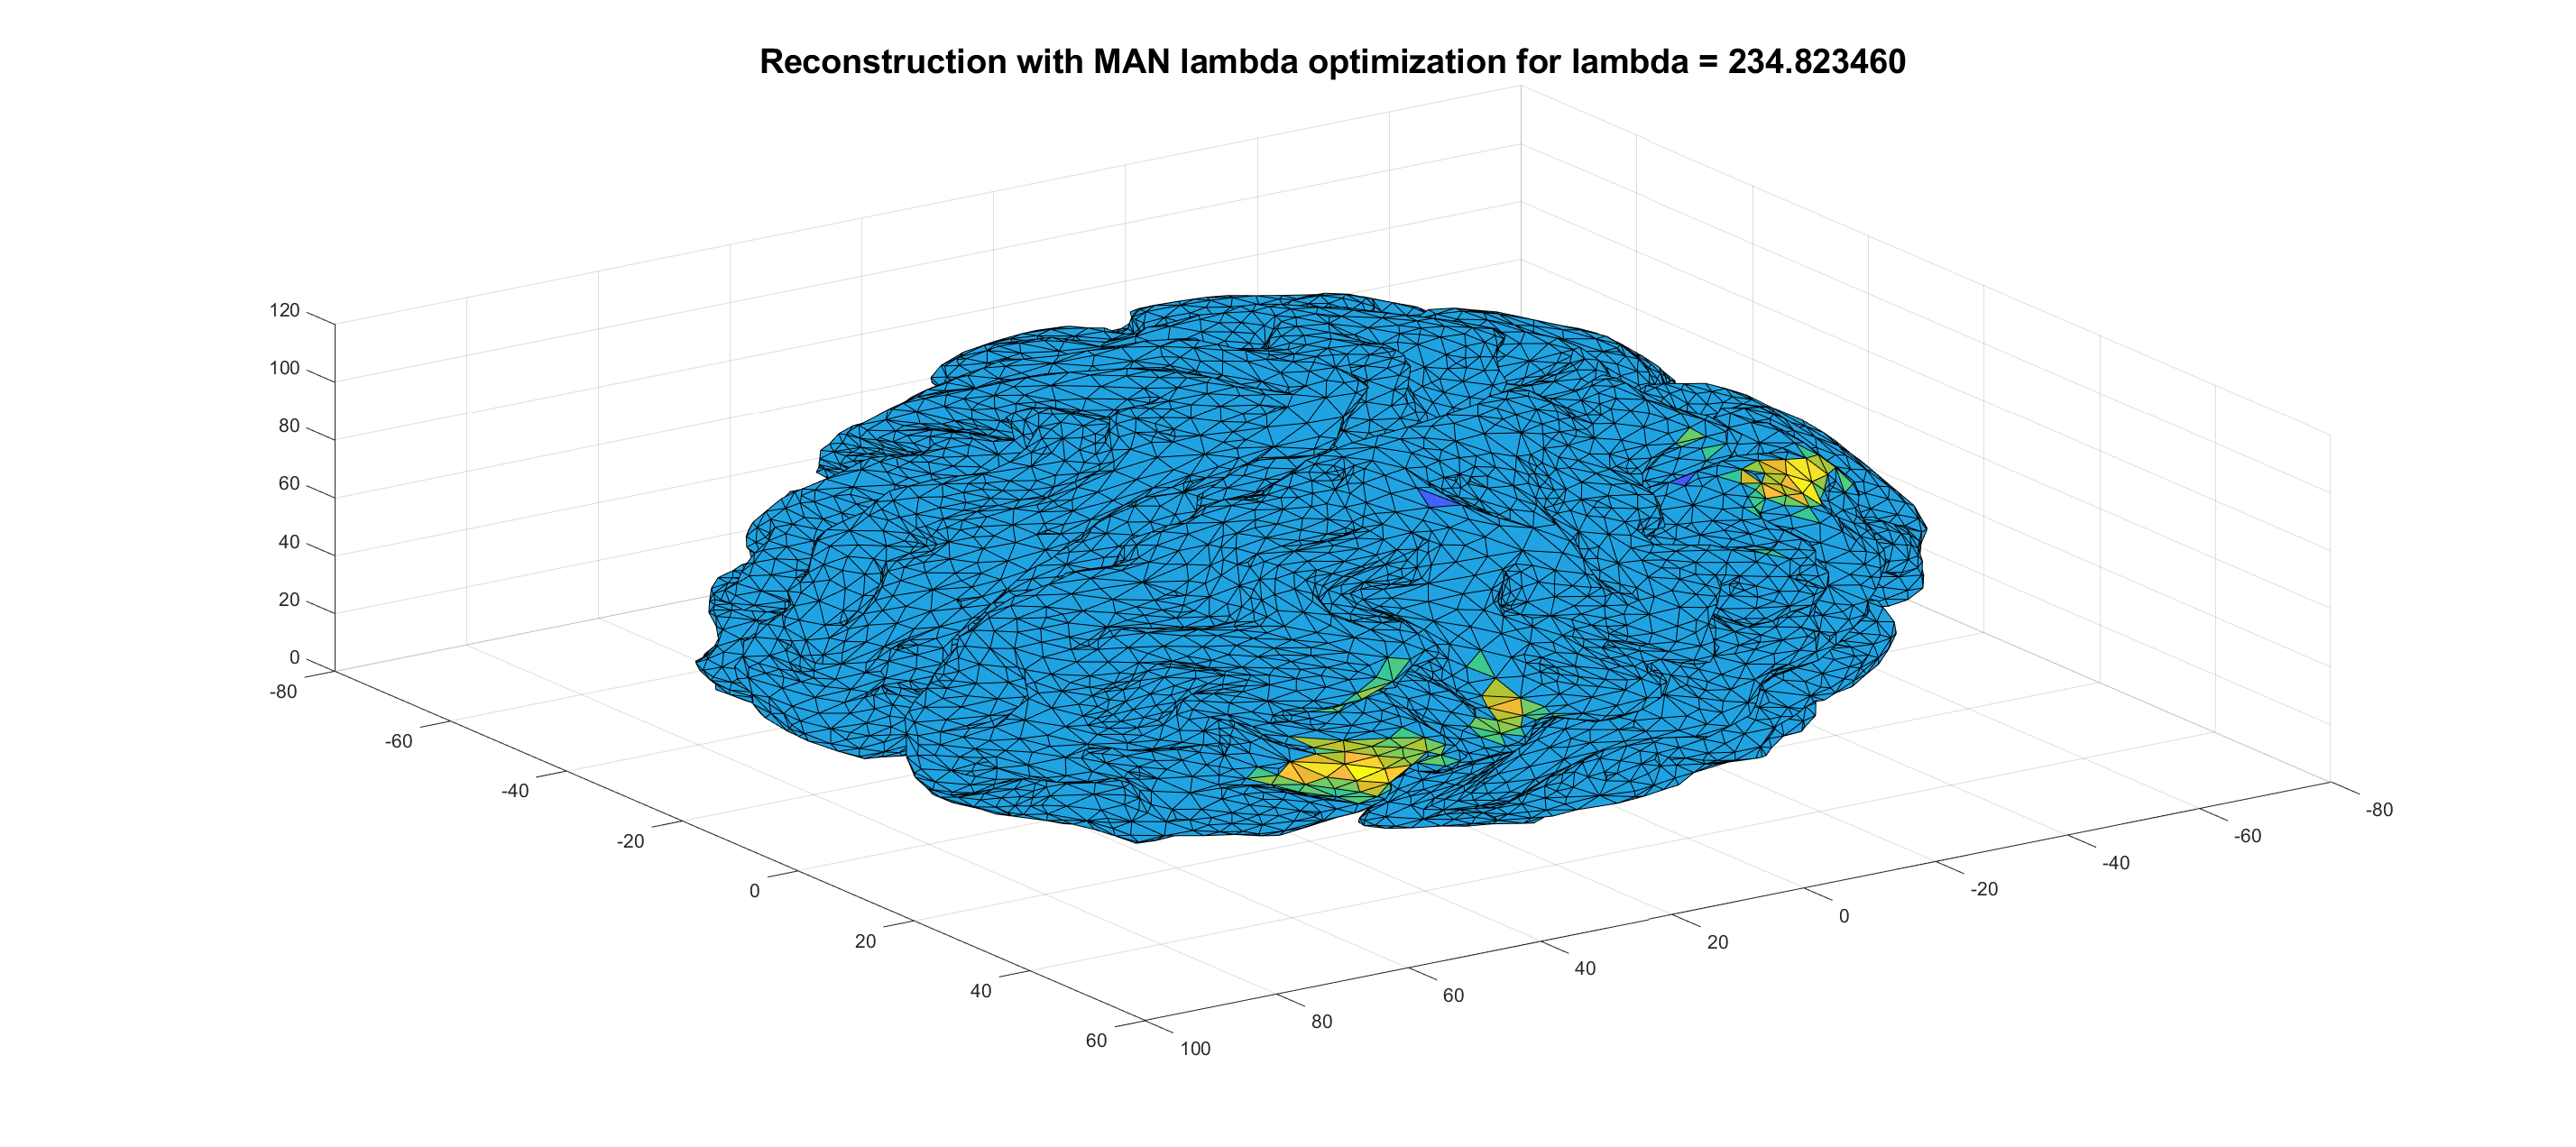
\includegraphics[width=.6\textwidth]{man_100}
    \centering
\end{figure}

\begin{figure}[H]
    \caption{Méthode L-curve}
    \label{brain}
    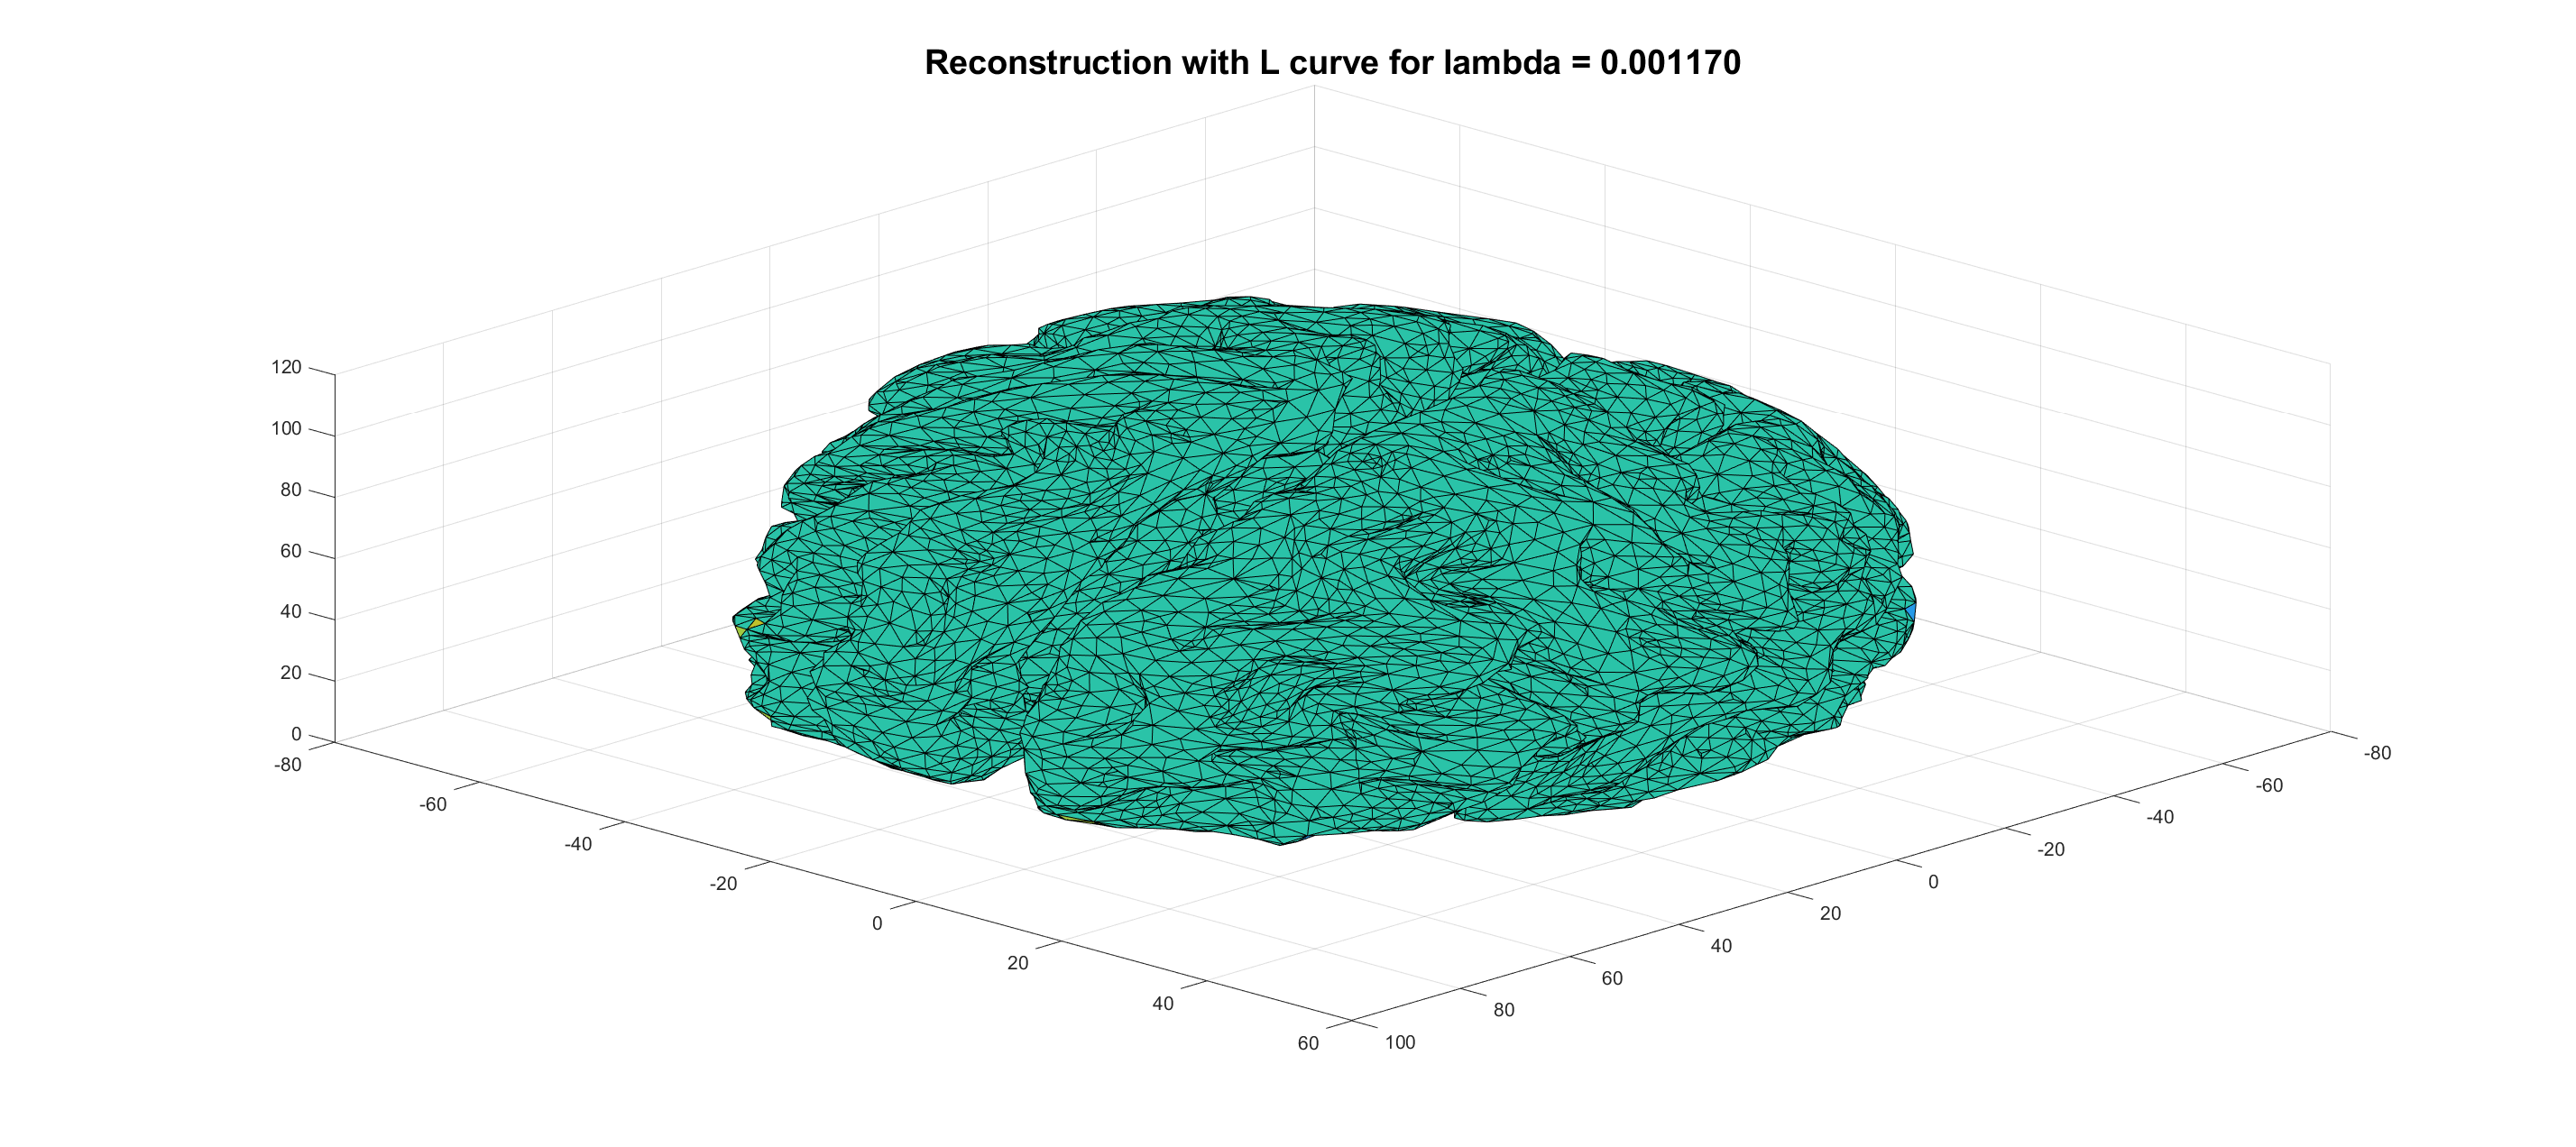
\includegraphics[width=.6\textwidth]{l_100}
    \centering
\end{figure}

\begin{figure}[H]
    \caption{Méthode DISC}
    \label{brain}
    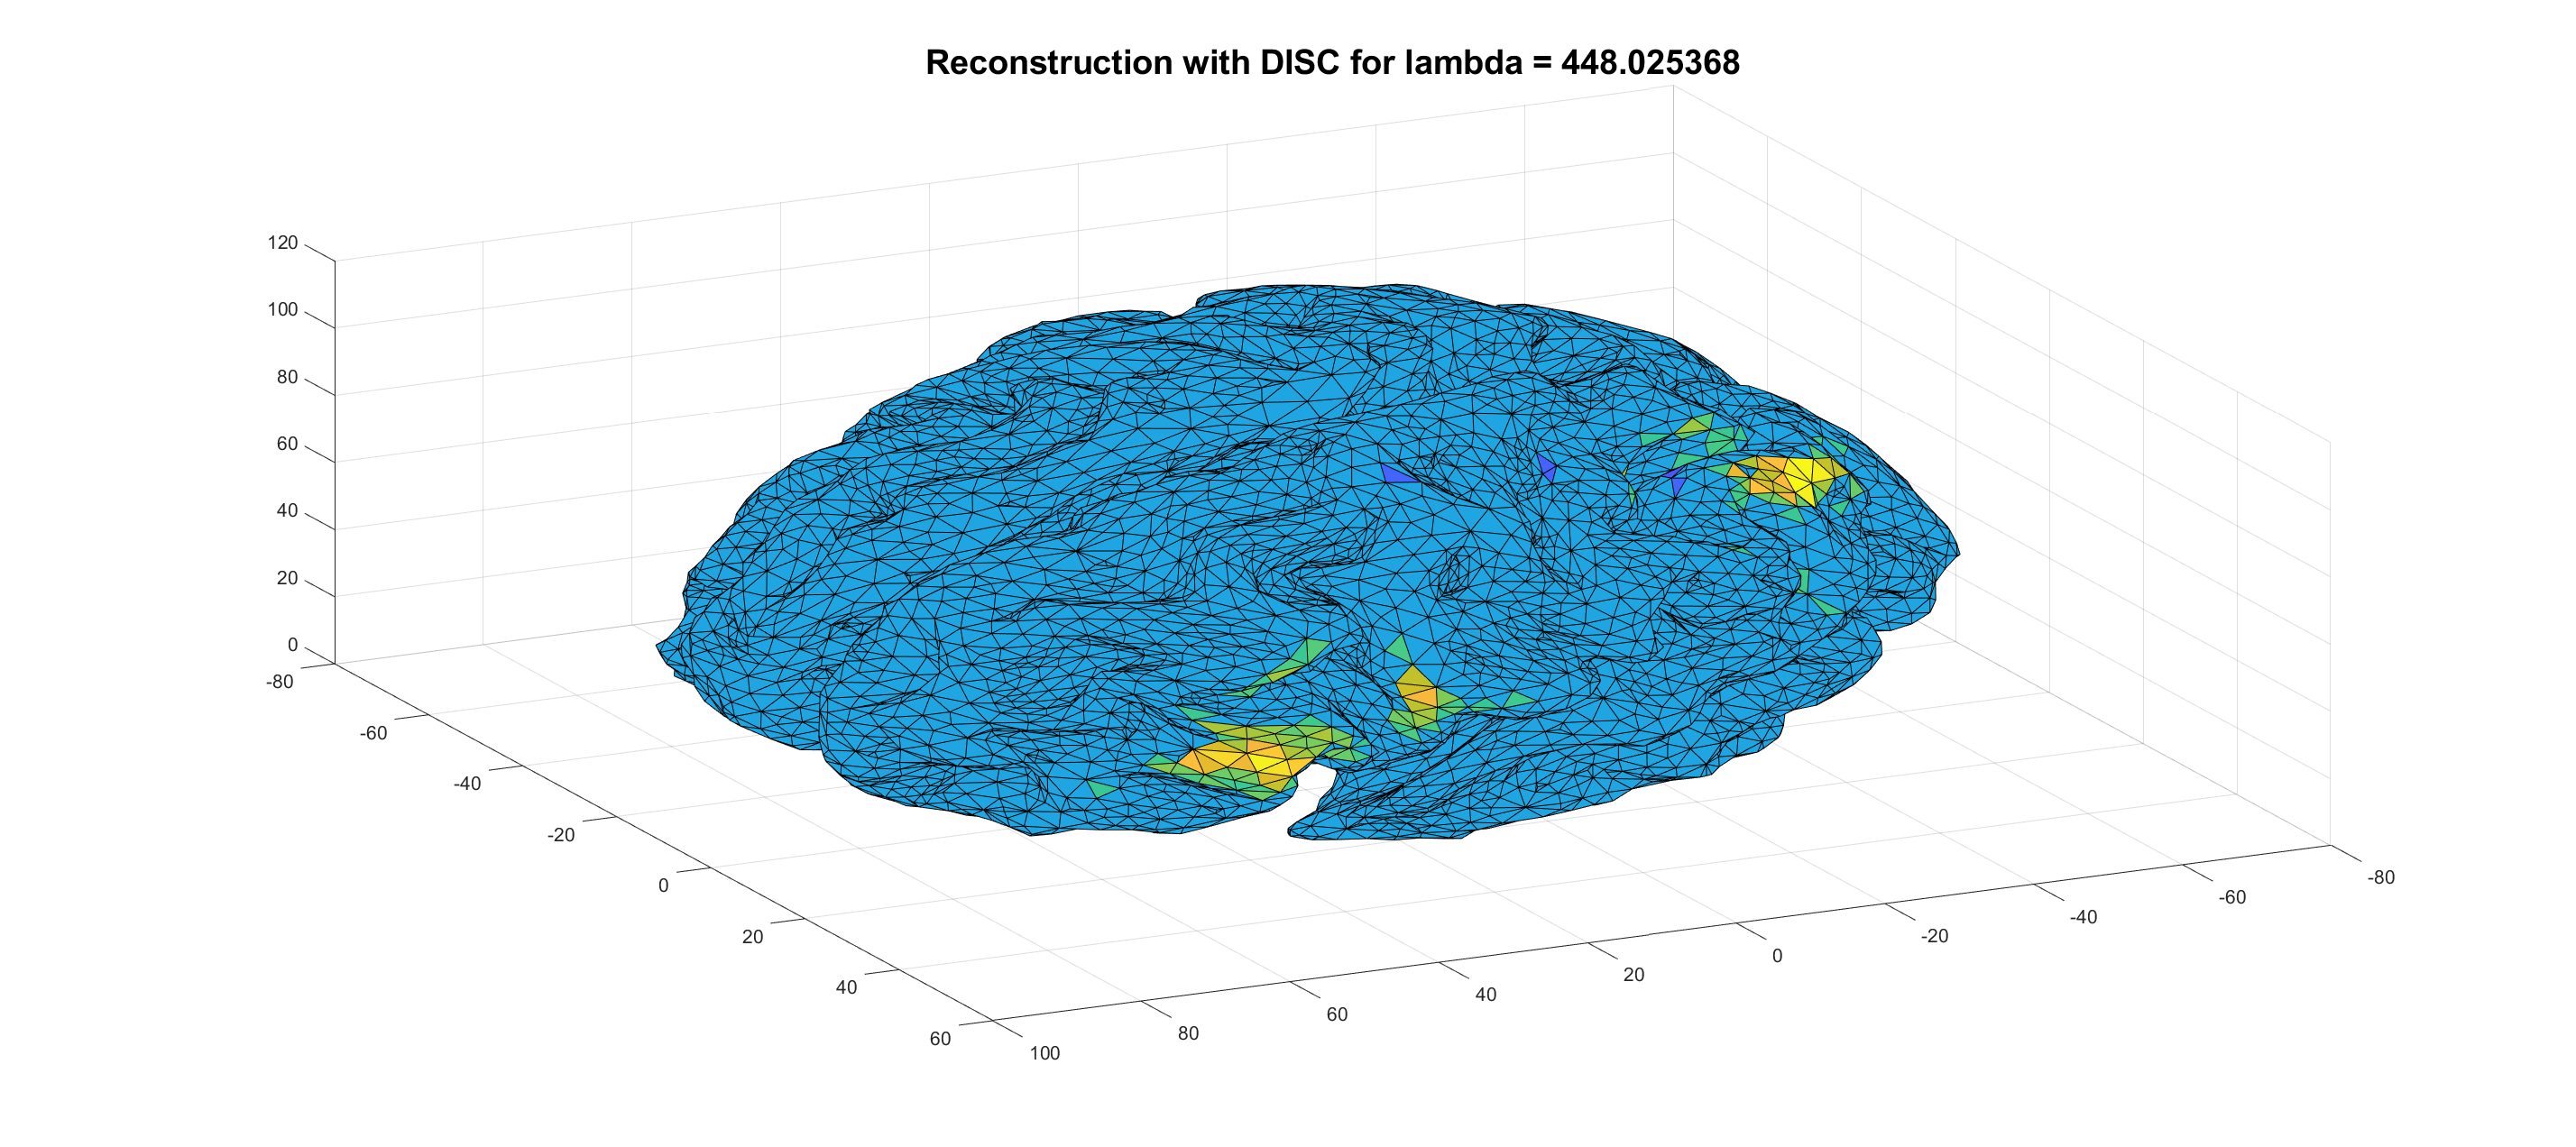
\includegraphics[width=.6\textwidth]{disc_100}
    \centering
\end{figure}

On observe alors que :

\begin{itemize}
    \item{Pour les différentes valeurs du RSB, chaque méthode fournit des résultats
        qui différent des autres}
    \item{Dans ce cas, on observe que la méthode DISC fournit les meilleurs résultats,
        suivie de la méthode manuelle et enfin de la méthode L-curve. Cependant, on ne peut
        pas en déduire un classement général des méthodes.}
    \item{Enfin, ajuster les seuil pourrait nous permettre d'observer des images plus proches
        de la vérité terrain pour les différents cas}
\end{itemize}

\section*{Conclusion}

Ainsi, au cours de ce TP nous avons pu nous intéresser au problème de la localisation de sources
en EEG. Nous nous sommes focalisé sur la régularisation de Tikinnov et avons pu implémenter
trois méthodes pour le choix du paramètre de régularisation : manuelle, L-curbe et DISC.

Nous avons pu alors prendre conscience de la complexité du problème. En effet, en pratique,
nous ne disposons pas de vérité terrain pour pouvoir évaluer nos résultats. De plus, le choix
du paramètre de régularisation est complexe Nous n'avons pu exhiber aucune méthode simple nous
permettant de toujours choisir la meilleure valeur. Au contraire, il faut plutôt essayer
différentes méthodes et sélectionner celle qui nous semble fournir le meilleur résultat
pour un problème donné. De plus, la valeur du seuil doit également être ajustée pour
obtenir de bons résultats.

\end{document}
